% File tacl2018v2.tex
% Sep 20, 2018

% The English content of this file was modified from various *ACL instructions
% by Lillian Lee and Kristina Toutanova
%
% LaTeXery is mostly all adapted from acl2018.sty.

\documentclass[11pt,a4paper]{article}
\usepackage{times,latexsym}
\usepackage{url}
\usepackage[T1]{fontenc}

%% Package options:
%% Short version: "hyperref" and "submission" are the defaults.
%% More verbose version:
%% Most compact command to produce a submission version with hyperref enabled
%%    \usepackage[]{tacl2018v2}
%% Most compact command to produce a "camera-ready" version
%%    \usepackage[acceptedWithA]{tacl2018v2}
%% Most compact command to produce a double-spaced copy-editor's version
%%    \usepackage[acceptedWithA,copyedit]{tacl2018v2}
%
%% If you need to disable hyperref in any of the above settings (see Section
%% "LaTeX files") in the TACL instructions), add ",nohyperref" in the square
%% brackets. (The comma is a delimiter in case there are multiple options specified.)

\usepackage[]{tacl2018v2}

\usepackage{booktabs}
\usepackage{pifont}
\usepackage{url}
\usepackage{amsmath}
\usepackage{amssymb}
\usepackage{multirow}
\usepackage{xspace}
\usepackage{soul}
\usepackage{subcaption}
\usepackage{epsfig,endnotes,graphicx,subcaption,xspace}
\usepackage{enumitem}
\usepackage{hyperref}
\usepackage{float}

%%%% Material in this block is specific to generating TACL instructions
\usepackage{xspace,mfirstuc,tabulary}
\newcommand{\dateOfLastUpdate}{Sept. 20, 2018}
\newcommand{\styleFileVersion}{tacl2018v2}

\newcommand{\ex}[1]{{\sf #1}}

\newcommand*{\img}[1]{%
    \raisebox{-.1\baselineskip}{%
        \includegraphics[
        height=0.8\baselineskip,
        width=0.8\baselineskip,
        keepaspectratio,
        ]{#1}%
    }%
}

\newif\iftaclinstructions
\taclinstructionsfalse % AUTHORS: do NOT set this to true
\iftaclinstructions
\renewcommand{\confidential}{}
\renewcommand{\anonsubtext}{(No author info supplied here, for consistency with
TACL-submission anonymization requirements)}
\newcommand{\instr}
\fi

%
\iftaclpubformat % this "if" is set by the choice of options
\newcommand{\taclpaper}{final version\xspace}
\newcommand{\taclpapers}{final versions\xspace}
\newcommand{\Taclpaper}{Final version\xspace}
\newcommand{\Taclpapers}{Final versions\xspace}
\newcommand{\TaclPapers}{Final Versions\xspace}
\else
\newcommand{\taclpaper}{submission\xspace}
\newcommand{\taclpapers}{{\taclpaper}s\xspace}
\newcommand{\Taclpaper}{Submission\xspace}
\newcommand{\Taclpapers}{{\Taclpaper}s\xspace}
\newcommand{\TaclPapers}{Submissions\xspace}
\fi

%%%% End TACL-instructions-specific macro block
%%%%

%%%% Our macros %%%%
\newcommand{\eat}[1]{}

\newcommand{\nb}[1]{\textcolor{blue}{$_{NB}${[#1]}}}



\title{Towards Extracting Formal Models from Specifications: A dataset, challenges, and other resources.}

% Author information does not appear in the pdf unless the "acceptedWithA" option is given
% See tacl2018v2.sty for other ways to format author information
\author{
 Template Author\Thanks{The {\em actual} contributors to this instruction
 document and corresponding template file are given in Section
 \ref{sec:contributors}.} \\
 Template Affiliation/Address Line 1 \\
 Template Affiliation/Address Line 2 \\
 Template Affiliation/Address Line 2 \\
  {\sf template.email@sampledomain.com} \\
}

\date{}

\begin{document}
\maketitle
\begin{abstract}


\end{abstract}

\section{Introduction}

\section{Tests for \MfR}
A good \mfr is one where information from all the facts are used to arrive at the answer. How can we test for this? Previous work has identified two properties of \mfr that can be tested using simple prediction tasks. 

\begin{enumerate}
\item Finding the correct answer -- All \mf datasets include questions that supposedly require information from two or more facts to answer. A valid \mfr solution will arrive at the correct answer for these questions. Given a question and the input text context ($Q$, $C$), the task is to output the correct answer $A$. 

\item Finding the supporting facts -- A valid \mfr solution will have used information from the correct supporting facts to arrive at its answer. Given a question and the input text context ($Q$, $C$), the task is to output all the supporting facts $F_s$ in $C$.
\end{enumerate}

However, because of biases and artifacts in the datasets, models can pass these tests without having to use information in all of the supporting facts. In particular, in most \mf datasets the input context always has correct answer and all supporting facts within it. In this case, the support identification reduces to supporting \textit{facts} identification, where as long as models can identify (locate) the supporting facts, they get a point. This means models do not need to know whether these supporting facts are {\em sufficiently} supporting the answer. \nb{The last two sentences of this paragraph are not clear to me. I think I get the high level point but the impact of reduction to support identification needs to come through for the argument to make sense.}
\tk{I really like this reduced version. But I also feel that the motivation for sufficiency is weaker now. Maybe just one line about how these metrics can be ``cheated'' by non-MF models?}

\subsection{Contrastive Support Sufficiency Test}

\nb{To mitigate this problem, we add another \nb{test} which we call sufficiency prediction, in which the model needs to identify whether there is sufficient support in the context to arrive at the answer. A similar test has been used to Squad 2.0, as unanswerable but ....(list the issues w doing it this way). To avoid introducing new artifacts we propose a testing procedure that relies on the availability of labeled supporting facts.}

Importantly, we show an automatic way of constructing such instances by leveraging the supporting facts from the multi-fact QA dataset. We call refer to this as sufficiency-based transformation (SuTra), one that can be applied to any \mf dataset that has supporting fact annotations for each question.

\harsh{I think we should explain first that we can expect humans to tell whether enough evidence is available in text or not for the question to be answerable. Then say that under our {\bf assumed} annotation of supporting facts, humans would consider any proper subset of supporting facts as insufficient for the question to be answerable. Unless we don't bring in expectation from a human, the specific task detail might seem unmotivated.}
\nb{I don't want to bring in humans at all in any of this discussion, except in evaluation. Bringing in humans can cause a distraction in terms of how would humans reason about these questions etc.}

\subsection{Contrastive Support Sufficiency Transform}

Formally, given a question $Q$ and a collection of facts $C^{prime}$ from the original context $C$, the sufficiency test is to decide if $C^{\prime}$ contains all the supporting facts for answering the question. Given that we know the full set of supporting facts $F_s$ and assuming that information in them is not duplicated elsewhere in the original input context $C$, we can create many test cases for sufficiency. A test case where $C^{\prime}$ contains all supporting facts i.e., where $F_s \subseteq C^{\prime}$, is sufficient for answering the question, whereas a case where $C^{\prime}$ is missing at least one supporting fact i.e., where $C^{\prime}/F_s$ is non-empty is  insufficient. A model is deemed to pass the sufficiency test if and only if it makes the correct decision for every test case. To ensure we don't introduce length or other artifacts in creating these test cases, we use the following procedure to create these test cases.


\begin{figure}[t]
    \centering
	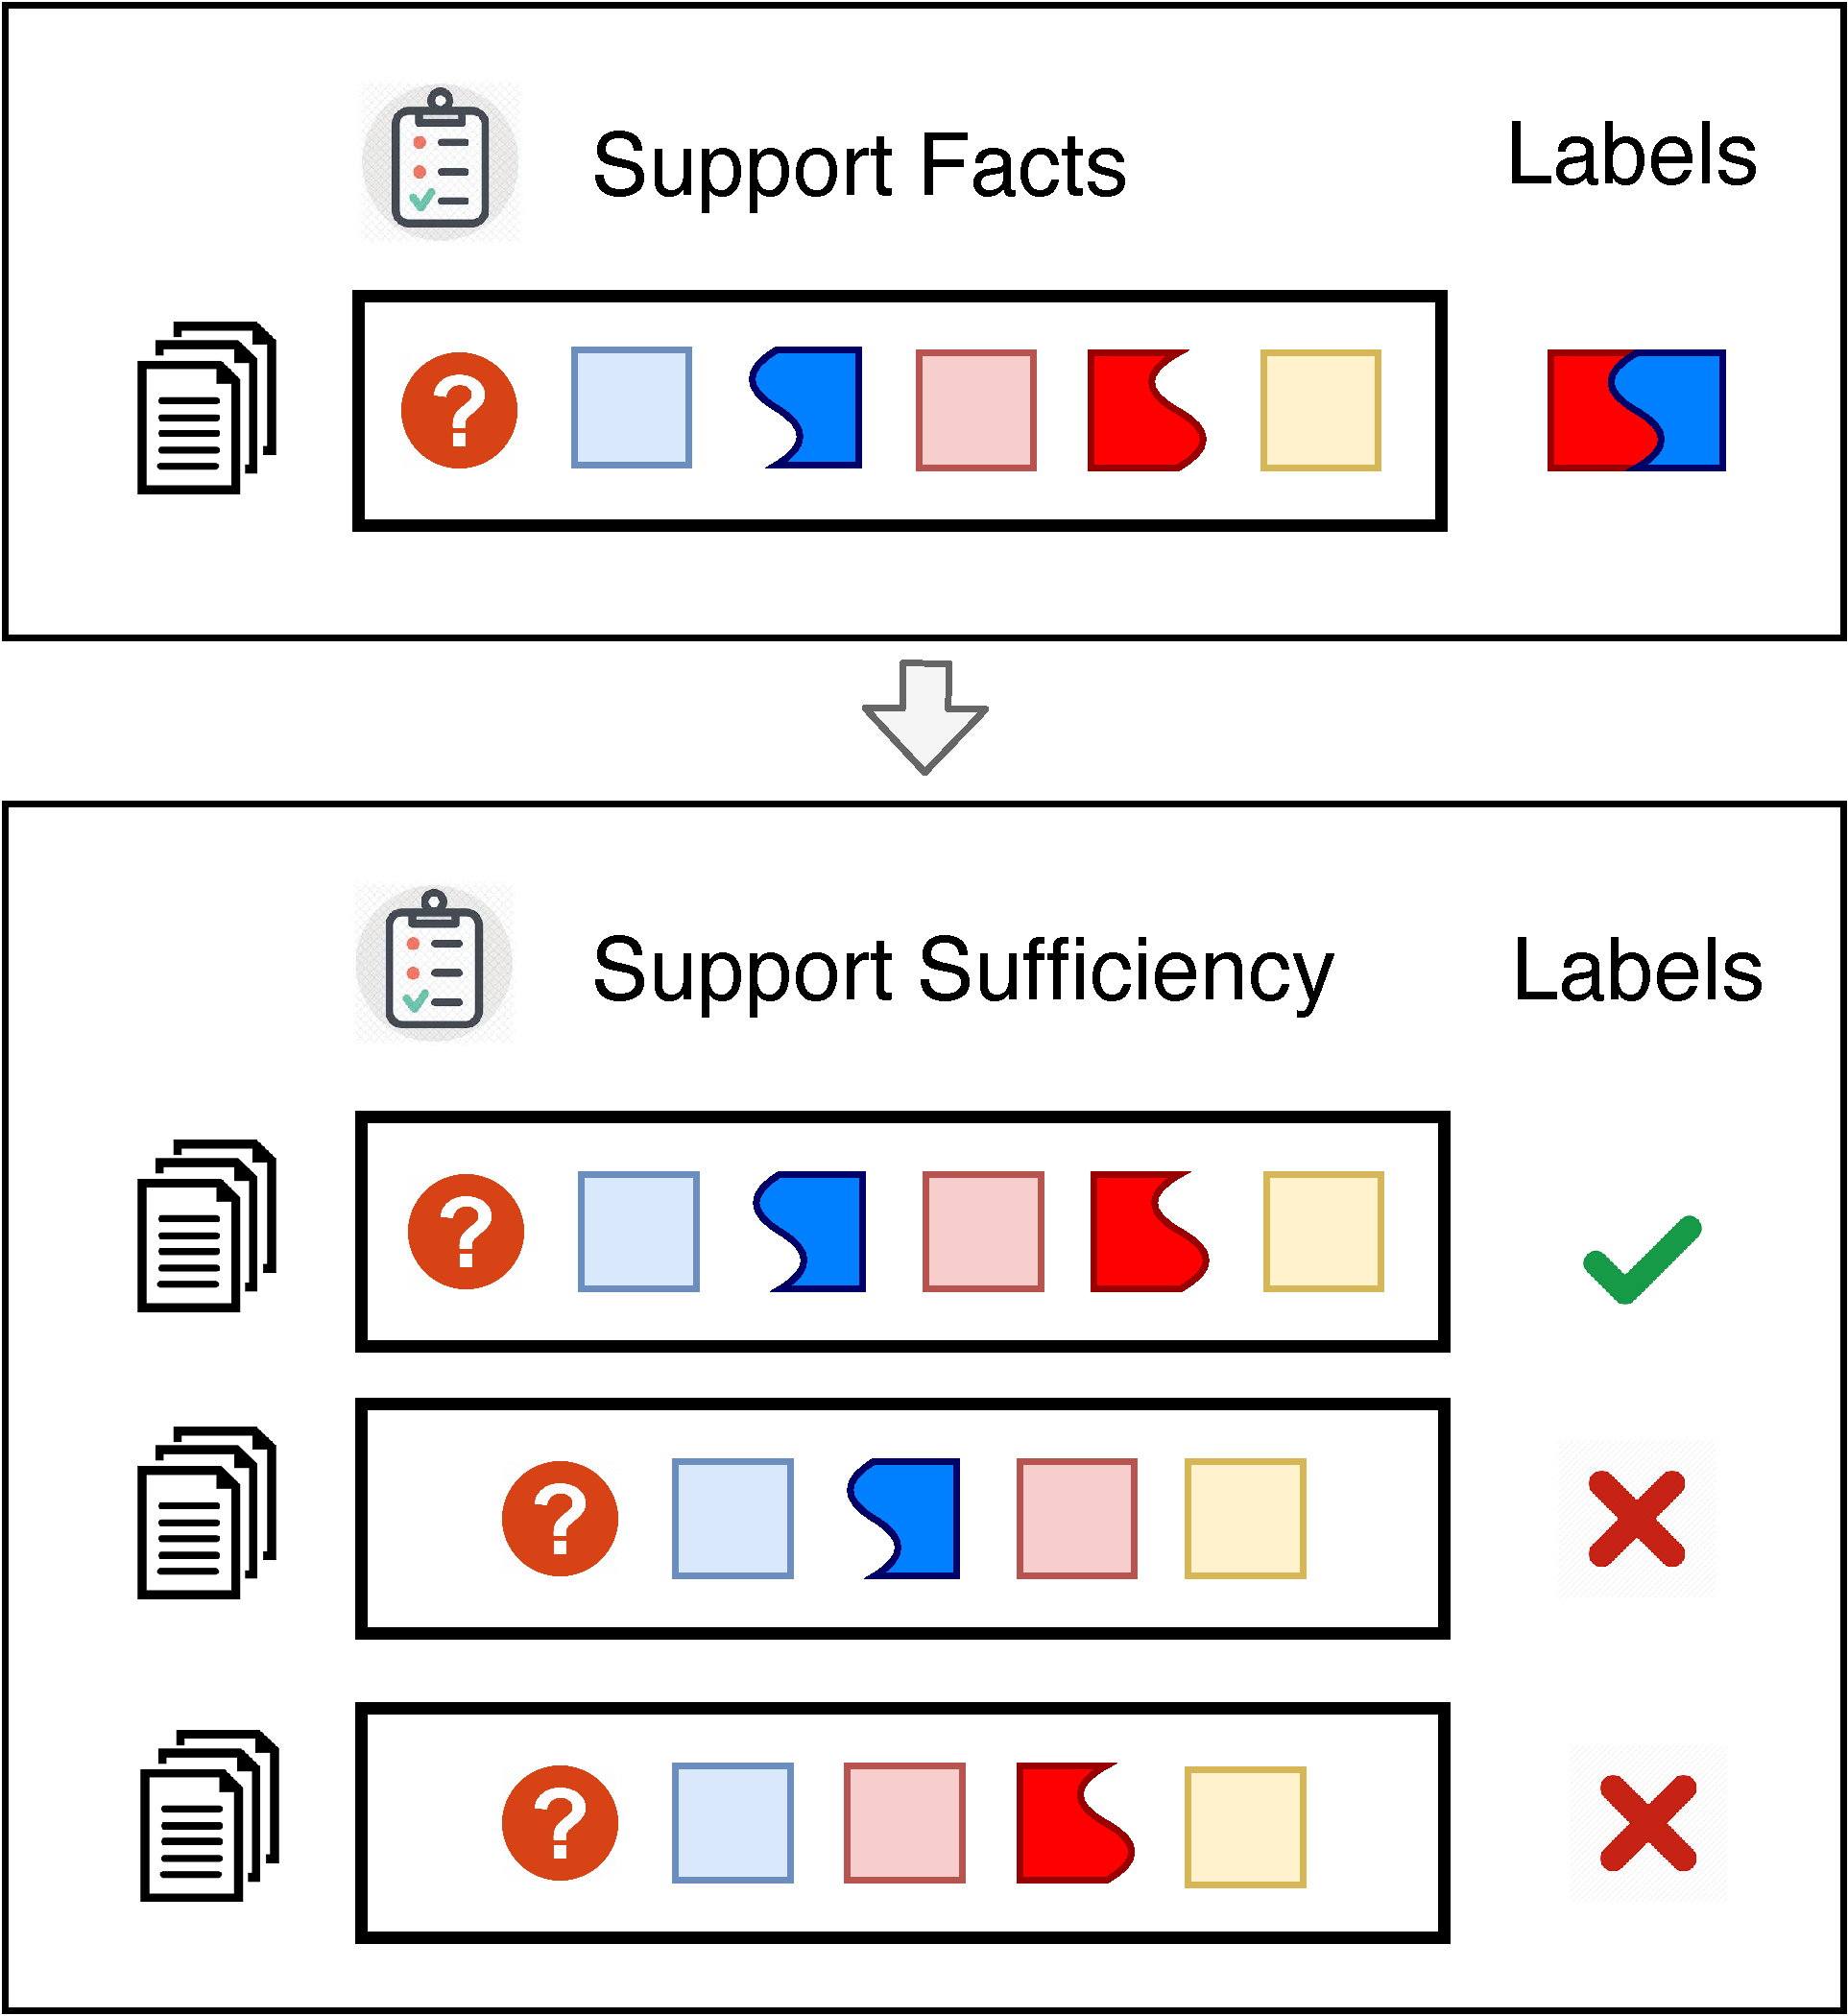
\includegraphics[width=0.35\textwidth]{images/transformation-v3}
	\caption{TODO: Explain why the support sufficiency prediction is harder than support location.}
	\label{fig:intro}
\end{figure}

%a subset of facts in the input context, i.e., given some $C^{\prime} \subseteq C$, test if $C^{\prime}$ contains {\em all} the supporting facts that necessary for answering the question.

%contains \it{all} the sufficient\harsh{supporting?} facts $F_s$ \harsh{sufficient} to support the correct answer. 

%We assume that the information in $F_s$ is not duplicated elsewhere in $C$. \harsh{Here, I think (i) we can say that task to test from some context $C$ itself. We use $C^{\prime} \subseteq C$ just to balance out the number of facts in positive and negative examples, but that's an implementation/method detail that we are anyway explaining later. (ii) I think if we say, "test if C contains all supporting facts", it won't be clear that it's all vs none, all vs partial or we annotate examples like Squad2. I think we need something that highlights this all vs partial check to separate what we are doing from general notion of unanswerable questions in Squad2 and others.}

\nb{Harsh, I am highly confident that I am wrong in what I have written below. Can you fix it?}

We first create sufficient context instances of a fixed size using all the sufficient facts $F_s$ and different subsets of other facts in $F_c$.
We create examples of insufficient contexts as follows. First, we create multiple (proper) subsets of the supporting facts. For each such proper subset $F_p$ we add some other facts from the original input context to create an insufficient context.\footnote{This process creates multiple negative instances for each positive instance. During training we balance the instances through under sampling but during test time we test on all negative examples since a model must be robust to all insufficient contexts.} We ensure that the size of the contexts is the same for both sufficient and insufficient cases.
\nb{Say something here that explains the equation below.}
\begin{itemize}[noitemsep]
    \item $(Q, F_s + F_d'; L_C=1)$
    \item $(Q, F_p + F_q + F_d'; L_C=0)$
\end{itemize}

A model passes the sufficiency test if and only if it is able to identify the sufficient and insufficient contexts in all cases. 

All of these \mfr tests, including sufficiency, can be hacked by \nmfr as long as there are artifacts and biases in the datasets. It turns out that we can measure how much models can score on these tests using \nmfr by devising probes 

%However, as we discuss in the next section, sufficiency test is significantly more difficult to hack in practice than the finding answer and supporting fact tests. Next, we show how we can turn these tests into probes for measuring \nmfr.


%Like answer and supporting fact tests, this support sufficiency test can also be hacked by non-multi-fact reasoning, but as we will discuss in the next section, that in practice, it's significantly less cheatable.

%Suppose that $F_s$ is the exact set of supporting facts in $C$ i.e., there exists no other subset of $C$ that duplicates information present in $F_s$.

%Assume that $F_s$ is the only support for humans to arrive at the answer for {\it Q} in {\it C}, i.e., the information crucial to arrive at the answer in any of the supporting facts $F_s$ is not duplicated in $F_d$. Under such a setting, we can automatically create instances where sufficient support is absent in the context and we can require the model to distinguish such instances with insufficient support from instances with sufficient support. Consider $F_p$ to be some proper subset of $F_s$. The context $F_p + F_d$ does not have sufficient support to answer the question, whereas $F_s + F_d$ has. So we can require the model to predict a binary class of sufficiency separating these two types of instances. Of course, we also need to make sure we don't introduce new biases making this classification task trivial.

\eat{
\tk{Possibly getting into the details after this. Doesn't seem necessary at this point}\harsh{Note that this is the only place we are introducing + describing our sufficiency based transform. It's not described anywhere else. The later section talks about: given this sufficiency based predictable property how can it be hacked.}
%Concretely, consider $|F_s| = n$ and $|F_d| = m$ with $m>n$. We randomly sample $n-1$ facts from $F_d$ to form $F_r$ and call the remaining facts in $F_d$ as $F_d'$. We create a sufficient support context with $F_s + F_d'$. And for each proper subset $F_p$, we sample $n-k$ examples from $F_r$ to form $F_q$ and create insufficient support context with $F_p + F_q + F_d'$. Note that $|F_s+F_d'| = |F_p + F_q + F_d'|$. Taking $L_c$ as a label for sufficient support present or not, for $F_p \subset F_s$, we construct the following examples:

\begin{itemize}[noitemsep]
    \item $(Q, F_s + F_d'; L_C=1)$
    \item $(Q, F_p + F_q + F_d'; L_C=0)$
\end{itemize}

We do this for all proper subsets of $F_s$ and the model gets a point if it exactly identifies the sufficiency classification for \textit{all} variations generated from independent of each other. \harsh{IMP:} The model needs to make decision on each variation independent of others. Note that for all the variations the positive example is the same. At training time, we sample only one negative example for each each question to balance the dataset and at test time, we test it on all subset variations.

In practice, we propose a sufficiency-based transform that requires the model to predict all the three properties - answer, supporting facts and support sufficiency. We care about answer and relevance prediction only in the positive examples of sufficiency. The model gets a point if it gets a point in all of the individual properties.

The insufficiency prediction can be compared unanswerability of questions in SQUAD 2.0 which has been used to reduce reliance of models on superficial surface-level cues as pervasive in SQUAD 1.0. Importantly though, we propose an automatic way of constructing unanswerable questions and show it's link with multi-fact reasoning. Like answer and supporting fact properties, the support sufficiency is also cheatable by non-multi-fact reasoning, but we will discuss in the next section, that in practice, it's significantly less cheatable.


}

% \harsh{It's better to use "characterizing" instead of "defining" mf reasoning, given we know even if model is correctly predicting all the desired properties, it still doesn't imply good (multi-hop) "reasoning".}

% V1: 
% It is difficult to define \textit{what is good reasoning over text} in a quantifiable way given that we don't have a good understanding of how humans reason\cite{gardner2019making}. But we can characterize a good reasoning entity (model or human) to have an ability to answer a question in a QA task. This characteristic is although not a sufficient condition of good reasoning, is surely a necessary one. Like-wise it's also difficult to define \textit{what is good multi-hop reasoning in a quantifiable way}. But we can characterize a good multi-hop reasoning entity (model or human) to have an ability to predict certain attributes about the multi-hop solution that it is intended to take. One of such attributes that have been widely used in multi-hop reasoning research is identification of supporting (relevant) facts. Again, this characteristic is not a sufficient condition of good multi-hop reasoning, but is surely a necessary one.

% V2:
\eat{
Textual multi-fact reasoning can broadly be defined as the ability of an entity (human or machine) to aggregate and synthesize together information from different textual facts in a ``meaningful" way that generalizes to novel combinations of textual facts\tk{We don't seem to talk much about how this ``meaningful'' combination leads to generalization, I think. It might be okay to drop ``that generalizes...'' part}. One way of estimating the (multi-fact) reasoning abilities of a system is through the task of (multi-fact) question answering posed in given textual context. 

Concretely, we assume a multi-fact question answering dataset, where question {\it Q} in a dataset {\it D} has an associated context {\it C} and the correct answer is {\it A}. The context {\it C} is a set of facts $C = F_s + F_d$, where annotated $F_s$ is a set of supporting facts and $F_d$ is a set of distractor facts\footnote{A \textit{fact} is any continuous text like paragraph or sentence.}. We assume a human can answer the question by synthesizing at least some information from \textit{all} the supporting facts in a known subset of facts. \tk{Rather than tying this too annotations, which can be noisy, what if we instead talk in terms of some set of supporting facts? E.g. C is a set of facts that contains a set of supporting facts needed to answer the question, $F_s$ (and the rest are considered distractor facts $F_d$)}


Given this setup, we can expect a good reasoning entity (model or human) to have an ability to be able to predict the answer to the questions, and also predict certain attributes for an arbitrary question about the multi-fact solution that it is intended to take to arrive at the answer from the question \tk{Was hard to parse. Maybe ``Given this setup, we can expect a good reasoning entity (model or human) to be able to predict the answer as well as certain properties indicating the solution to arrive at the answer for any question.''.}. We call everything we expect models to predict on a QA instance a predictable property of the instance.

Two such properties which have been used in (multi-fact) QA research are: \\

\noindent \textbf{Answer Prediction:} Given instance input {\it (Q, C)}, the model should be able to predict associated answer {\it A}. Using $P_a$ to denote the answer property label, the input output behavior we expect is $(Q, C) \Rightarrow P_a{=}A$. The system gets a point on given question-context pair for answer property only if it predicts the answer exactly correctly. \\

\noindent \textbf{Supporting Facts Prediction} Given instance input {\it (Q, C)}, the model should be able to predict associated set of supporting facts $F_s$. Using $P_s$ to denote the supporting facts property label, the input output behavior we expect is $(Q, C) \Rightarrow P_s{=}F_s$. The system gets a point on given question-context pair for supporting facts property only if it predicts the whole set of supporting facts exactly correctly.

Although ability to predict such properties is a desirable one, it does not imply good reasoning owing to various biases and artifacts present in the dataset that pave shortcuts for models to predict the property correctly without the intended reasoning. \tk{We mention these biases/artifacts few times now. So a natural question would be: Shouldn't we try to remove these artifacts? Or does our transformation get rid of artifacts?}

The properties, answer and supporting facts are especially hackable because the model can assume that the answer and both the supporting facts are also present in the context. In this case, the support identification reduces to supporting \textit{facts} identification, where as long as models can identify (locate) the supporting facts, it gets a point. This means it does not need to know whether these supporting facts are sufficiently supporting the answer. 

To mitigate this problem, we propose to add another property which we call sufficiency prediction, in which the model needs to identify whether sufficient support is present in the context to arrive at the answer. Importantly, we show an automatic way of constructing such instances by leveraging the supporting facts from the multi-fact QA dataset. \\

\noindent \textbf{Support Sufficiency Prediction:} Assume that $F_s$ is the only support for humans to arrive at the answer for {\it Q} in {\it C}, i.e., the information crucial to arrive at the answer in any of the supporting facts $F_s$ is not duplicated in $F_d$. Under such a setting, we can automatically create instances where sufficient support is absent in the context and we can require the model to distinguish such instances with insufficient support from instances with sufficient support. Consider $F_p$ to be some proper subset of $F_s$. The context $F_p + F_d$ does not have sufficient support to answer the question, whereas $F_s + F_d$ has. So we can require the model to predict a binary class of sufficiency separating these two types of instances. Of course, we also need to make sure we don't introduce new biases making this classification task trivial.

\tk{Possibly getting into the details after this. Doesn't seem necessary at this point}\harsh{Note that this is the only place we are introducing + describing our sufficiency based transform. It's not described anywhere else. The later section talks about: given this sufficiency based predictable property how can it be hacked.}
Concretely, consider $|F_s| = n$ and $|F_d| = m$ with $m>n$. We randomly sample $n-1$ facts from $F_d$ to form $F_r$ and call the remaining facts in $F_d$ as $F_d'$. We create a sufficient support context with $F_s + F_d'$. And for each proper subset $F_p$, we sample $n-k$ examples from $F_r$ to form $F_q$ and create insufficient support context with $F_p + F_q + F_d'$. Note that $|F_s+F_d'| = |F_p + F_q + F_d'|$. Taking $L_c$ as a label for sufficient support present or not, for $F_p \subset F_s$, we construct the following examples:

\begin{itemize}[noitemsep]
    \item $(Q, F_s + F_d'; L_C=1)$
    \item $(Q, F_p + F_q + F_d'; L_C=0)$
\end{itemize}

We do this for all proper subsets of $F_s$ and the model gets a point if it exactly identifies the sufficiency classification for \textit{all} variations generated from independent of each other. \harsh{IMP:} The model needs to make decision on each variation independent of others. Note that for all the variations the positive example is the same. At training time, we sample only one negative example for each each question to balance the dataset and at test time, we test it on all subset variations.

In practice, we propose a sufficiency-based transform that requires the model to predict all the three properties - answer, supporting facts and support sufficiency. We care about answer and relevance prediction only in the positive examples of sufficiency. The model gets a point if it gets a point in all of the individual properties.

The insufficiency prediction can be compared unanswerability of questions in SQUAD 2.0 which has been used to reduce reliance of models on superficial surface-level cues as pervasive in SQUAD 1.0. Importantly though, we propose an automatic way of constructing unanswerable questions and show it's link with multi-fact reasoning. Like answer and supporting fact properties, the support sufficiency is also cheatable by non-multi-fact reasoning, but we will discuss in the next section, that in practice, it's significantly less cheatable.

}
% Like answer and relevance prediction, sufficiency prediction is also not a a sufficient condition for good (multi-hop) reasoning, but is surely a necessary one. In the next section, we show how to capture the extent of information present in the dataset that paves shortcut to correct predictions.


% On such a dataset, a good reasoning model should be able to predict whether the information present in it is sufficient to answer the question or not. To automatically create positive and negative examples of binary classification of sufficiency we leverage the supporting facts annotation. The dataset only has positive examples of sufficiency. But for each positive example, we can create several negative example where the only supporting facts present in the context are proper subsets and not full set of annotated supporting facts. We further need to balance out the total number of facts in sufficient and insufficient examples to not inject this new bias that could make binary classification trivial.




% On such annotated dataset, a good reasoning entity (machine or human) should be able to predict the answer to arbitrary questions on the text. Furthermore, we can also expect a good multi-hop reasoning entity (model or human) to have an ability to predict certain attributes for an arbitrary question about the multi-hop solution that it is intended to take to arrive at the answer from the question. One such attribute that has been widely used in multi-hop reasoning research is identification of supporting (relevant) \ashish{This migth be the place to clarify: when datasets guarantee there is always full support present, \emph{support identification} reduces to the generally simpler task of \emph{relevance identification}, which we show is quite susceptible to NMF reasoning. However, when full support isn't guaranteed to be present, identifying whether full support is present is a strictly harder task than relevance identification, and a better assessment of multihop reasoning} facts which the system is intended to use and compose information from to arrive at the answer.

% The predictability of answer and relevance is not a sufficient condition for good (multi-hop) reasoning, but is surely a necessary one. This is because of various kinds of shortcuts exploitable by the model on the dataset task to evade the intended reasoning. Consider the example question \textit{"Which city was Facebook launched in?"} with two supporting facts (i)\textit{"Facebook was launched in Harvard."} and (ii)\textit{"Harvard is in \textbf{Cambridge} city."}, and some distracting facts. The intended reasoning here is to compose the information from the two supporting facts "meaningfully" to arrive at the answer and relevance predictions. However, depending on how the distracting the distracting facts are, a model can get both answer and relevance predictions right without any meaningful composition of facts that can generalize. For example, if there is no other mention of \textit{city} apart of supporting fact (ii), then answer and that supporting fact are easy to identify just through the question without any supporting fact composition. Similarly, if the supporting fact (i) is the only fact that has high overlap with the question, that relevant fact can also be identified through question and without any supporting fact composition. So both answer and (both) relevant facts can be identified without any meaningful supporting fact composition. The entity type matching and word overlap in the example here is just to give an intuitive notion of cheating. But the current generation of powerful pre-trained models are able to go far beyond such checks, allowing all of answer and relevance to be identified without any meaningful composition. This information can be misused by the model to "hack" the correct answer and relevance predictions.

% Such composition-less or interaction-less reasoning over supporting facts to hack answer and relevance prediction is fairly easily possible because models can assume that both the answer and both relevant facts are always present in the context. Removing this assumption, can mitigate such interaction-less reasoning (shortcuts) to a large extent. In the example above, we require the model to determine whether sufficient information is present in the context to answer the question or not based on whether \textit{both} supporting facts are present or not in the context, and if it is then further predict the answer and relevant facts. We will show in the later section that sufficiency prediction can also be hacked by interaction-less reasoning, but to a significantly lesser degree.

% We not that trivial AND can solve it if ....
% Model can no more make predictions in each part independent of other part. It has to do x.
% Most of the reasoning shortcuts in existing datasets arise due to the fact that the system can assume that the answer is guaranteed to exist in the given passage. Removing this assumption and
% requiring the system to identify whether the question is even answerable from the passage can prevent such shortcuts.

% One way of mitigating the problem is by requiring the models to determine the difference between the presence of both supporting facts and just one supporting fact in the set of facts as its context. The model now cannot do X
% One way of mitigating the problem is by requiring the models to separate out the difference of 

% TODO: Explain with example why answer and relevance both are fairly easily hackable in a way that directly motivates sufficiency prediction to mitigate this problem.


\section{Non-Multi-Fact Reasoning}

\subsection{Characterizing Non-Multi-fact Reasoning}

There can be various kinds of biases and artifacts present in the dataset that could pave shortcuts for models to predict the property correctly without the intended reasoning. In this work, we discuss about one kind of artifact (or bias) based reasoning that deals with \textit{multi-fact}edness of reasoning on multi-fact reasoning task. \harsh{I think this clarifies that in what we mean by non-multi-fact reasoning, the \textit{non} is on \textit{multi-fact}edness and not the \textit{reasoning}}

In a multi-fact QA dataset, the intended reasoning is to aggregate and synthesis together information from \textit{all} the supporting facts to arrive at the predicted conclusion. So we define non-multi-fact reasoning bias or artifact as the extent to which the information accessible by the model is present in the dataset to correctly predict all the task labels, without any non-trivial synthesis of information from \textit{all} the supporting facts.

Concretely, in a multi-fact QA dataset {\it D} with desired prediction property {\it P}, the extent of non-multi-fact reasoning bias accessible by the model {\it M} is measured by the maximum fraction of questions in {\it D} in which following conditions hold:

\begin{itemize}
    \item \textbf{Base condition:} model can predict exactly correctly {\it P} for the question.
    \item \textbf{NMF condition:} there exists at least one bi-partition of the supporting facts, such that without any \textit{non-trivial} synthesis of the two parts of the bi-partition among the context facts, the model can predict exactly correctly {\it P} for the question.
\end{itemize}

% \noindent \textbf{NMF Condition:} there exists at least one bi-partition of the supporting facts, such that without any \textit{non-trivial} synthesis of the two parts of the bi-partition among the context facts, the model can predict exactly correctly {\it P} for the question.

In practice, we probe NMF condition based on a re-written condition:

\noindent \textbf{NMF Condition:} there exists at least one bi-partition of the supporting facts, such that model predictions for property {\it P} of two parts of the bi-partitions (each part corresponds to the same context except without that supporting facts from that part) can be trivially combined together to predict exactly correctly {\it P} for the question.

\begin{figure}[t]
    \centering
	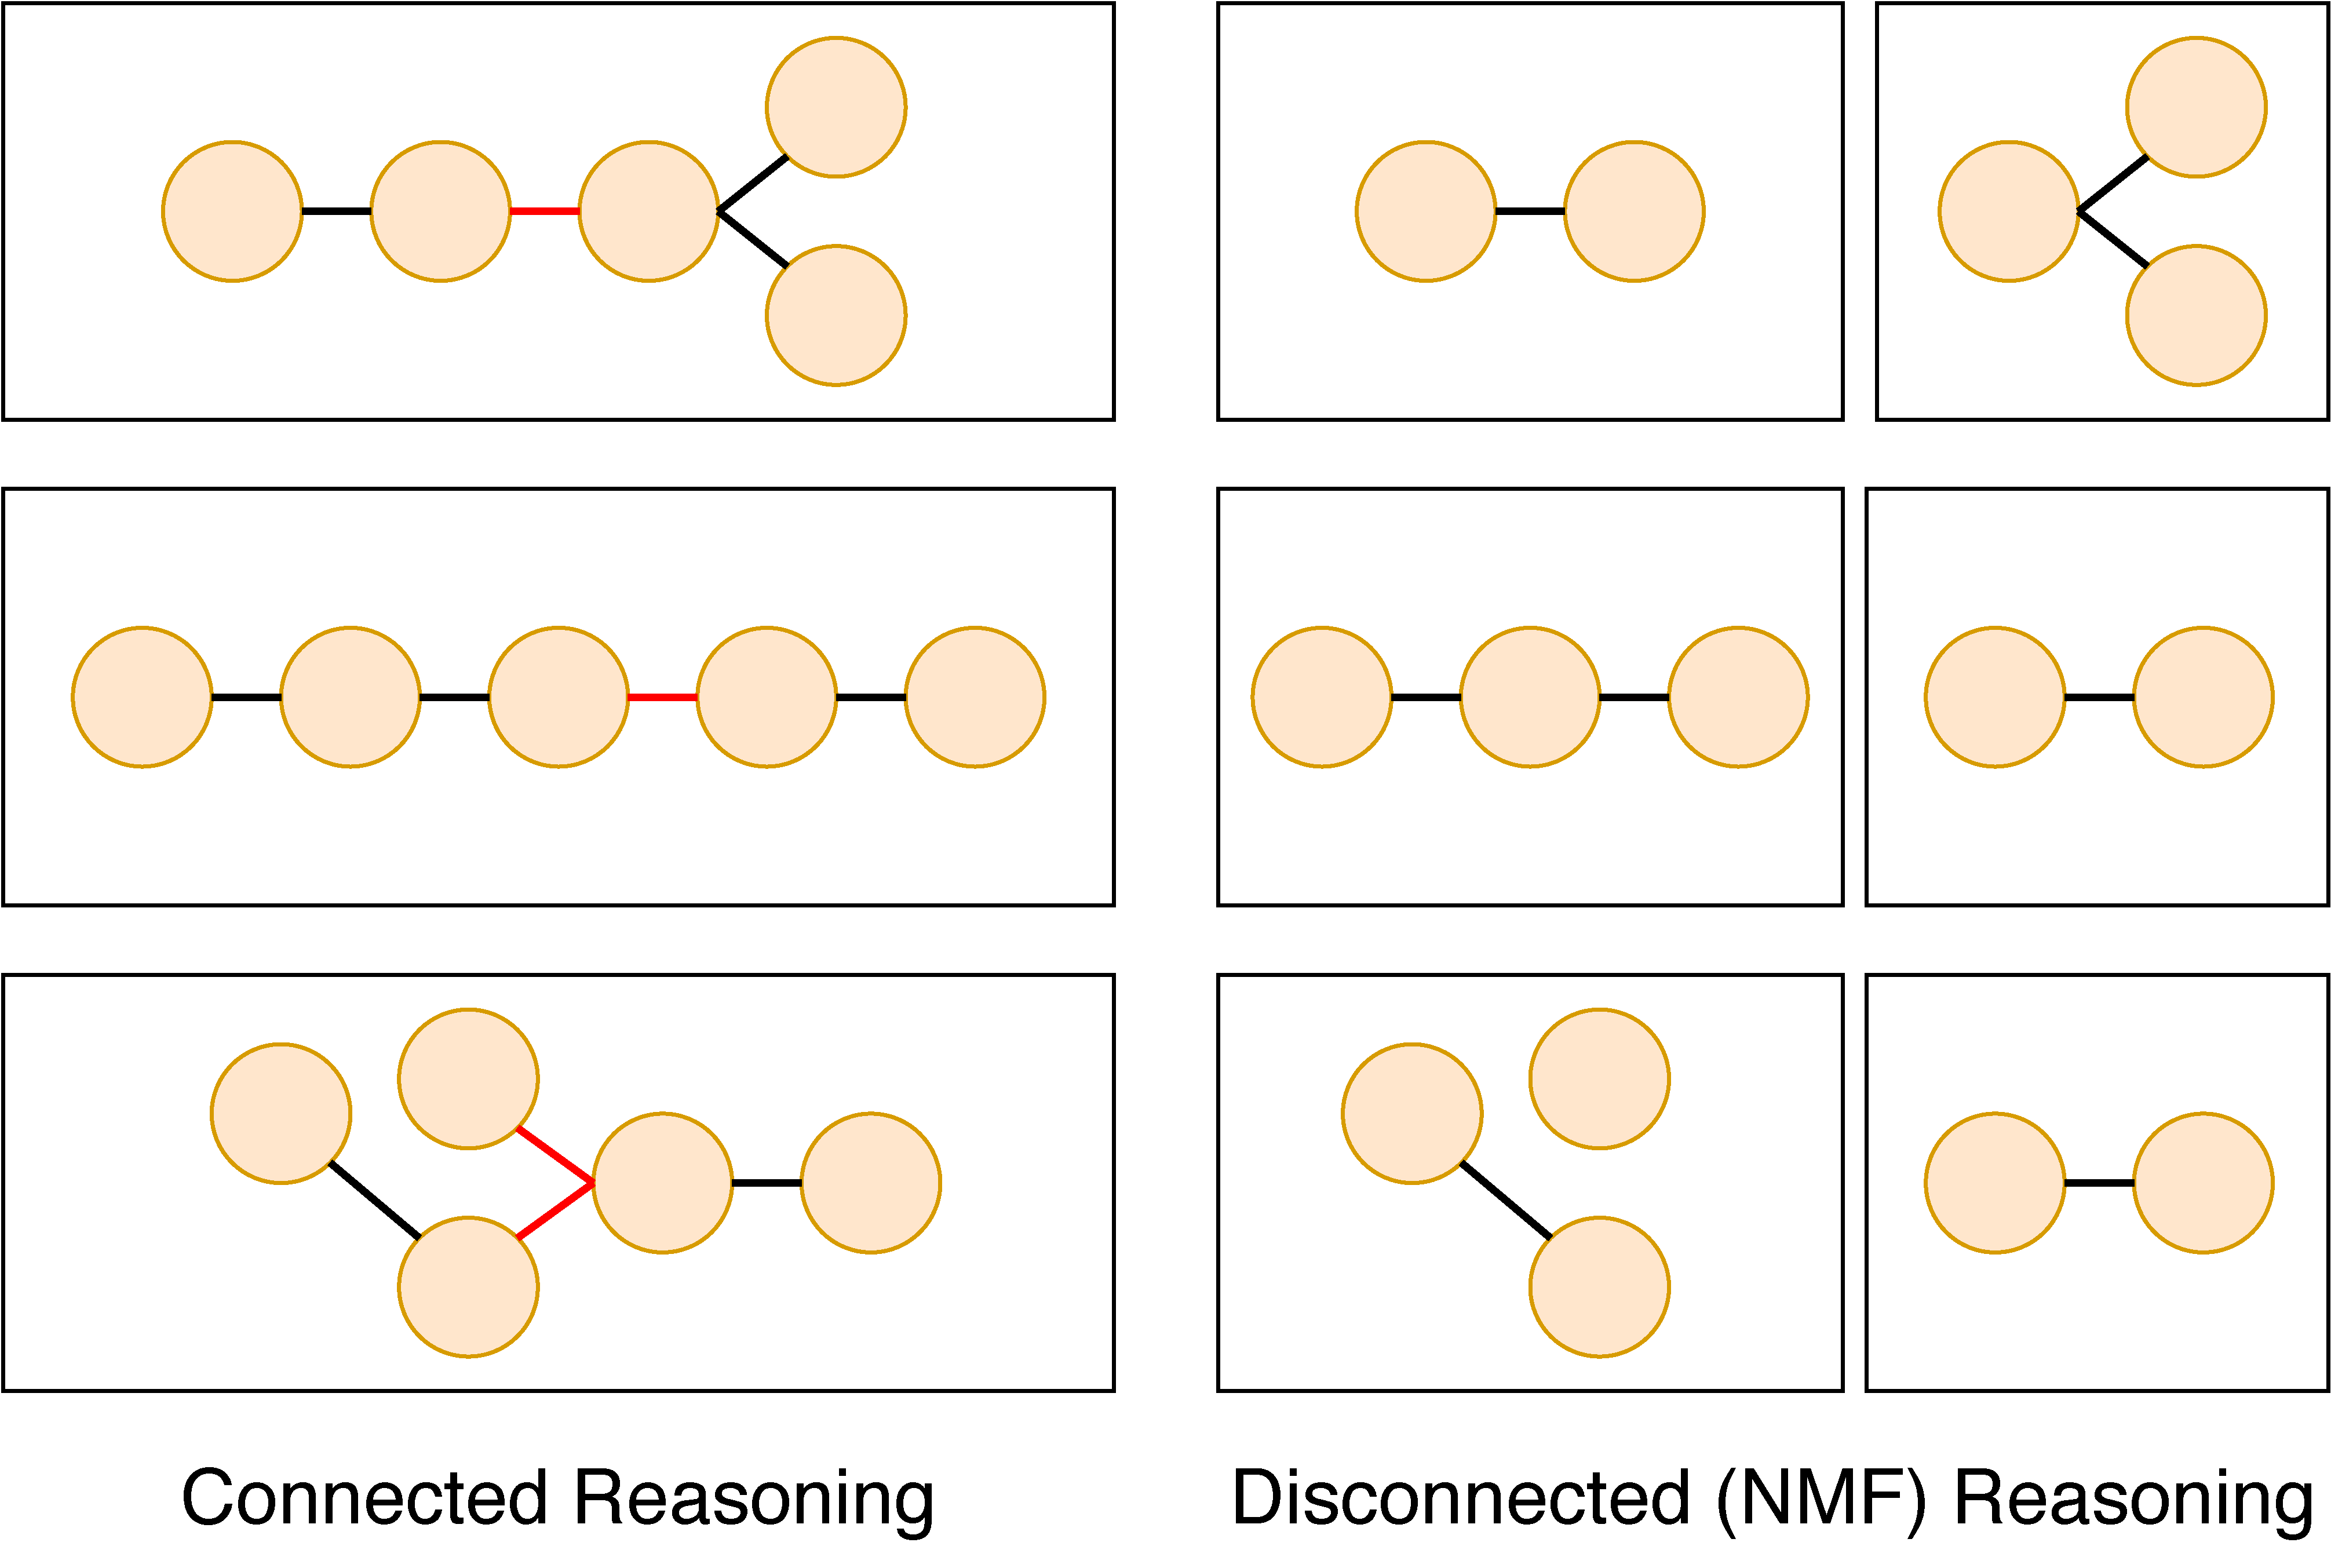
\includegraphics[width=0.45\textwidth]{images/factored-graph-v2}
	\caption{TODO: Explain }
	\label{fig:intro}
\end{figure}

Formally, for each property $P$, we want to check if the following is possible for some simple aggregation function $f_s$:

\begin{align}
     & P_r(P | (Q; F_{s_1} + F_{s_1} + F_d)) \nonumber  \\
    =& f_{s}\big(P_r(P | (Q; F_{s_1} + F_d)), P_r(P | (Q; F_{s_2} + F_d)) \big) \nonumber 
\end{align}

\harsh{Maybe the whole explanation of NMF reasoning can be explained in terms of factorization of joint probability distribution. Thoughts?}

We say that the multi-fact dataset property $P$ can be hacked by model $M$ with only non-multi-fact reasoning based on the maximum number of questions in which \textbf{Base} and \textbf{NMF} conditions hold.

We say that the amount of non-multi-fact reasoning a model could do as the fraction of maximum number of questions in which \textbf{Base} and \textbf{NMF} conditions hold to the maximum number of questions in which \textbf{Base} condition holds.

In \textbf{NMF} condition, we have used a notion of \textit{trivial combination}. Since the properties take various forms like span, set or list of items to name a few, it's difficult to define trivial combination in a completely property agnostic way. We instantiate the NMF condition for each property separately.


\subsubsection{Answer Prediction}

For input instance $(Q, C)$, the model should output answer $A$. But if there is a partition $(F_{s1}, F_{s2})$ of $F_s$ such that the model also correctly outputs $A$ on at least one of $(Q, F_{s1} + F_d)$ and $(Q, F_{s2} + F_d)$ as input, then we can say it is has information to do non-multi-fact reasoning for answer prediction.

\subsubsection{Supporting Fact Prediction}

For input instance $(Q, C)$, the model should output $L_s = F_s$. But if there is a partition $(F_{s1}, F_{s2})$ of $F_s$ such that the model also correctly outputs $F_{s1}$ in $(Q, F_{s1} + F_d)$ and $F_{s2}$ in $(Q, F_{s2} + F_d)$ as input, then we say it is has information to do non-multi-fact reasoning for supporting facts prediction.

\subsubsection{Support Sufficiency Prediction}

For input instance $(Q, C)$, the model should output $L_c = 0$ for \textit{every} variation of insufficient instance and sufficient instance for the question $Q$. But for \textit{every} subset of the supporting facts if it can differentiate between the presence and absence of the supporting facts among the distracting facts in the context, then it can decide $L_c$ labels for every variation without any synthesis of information from the supporting facts.

To see this, consider sufficient instance $(Q, F_s + F_d'; L_C=1)$ and a partition of $F_s$ as $F_{s1}$ and $F_{s2}$, and the corresponding insufficient instances $(Q, F_{s1} + F_{r1} + F_d'; L_C=0)$ and $(Q, F_{s2} + F_{r2} + F_d'; L_C=0)$. If the model can differentiate the inputs $(Q, F_{s1} + F_d')$ vs $(Q, + F_{r1} + F_d')$ and $(Q, F_{s2} + F_d')$ vs $(Q, F_{r2} + F_d')$, then it can predict the sufficiency labels ($L_C$) of \textit{all} three instance variations without any inter-dependence (\harsh{interaction might be confusing word here}) of supporting facts in $F_{s1}$ and $F_{s2}$. The same can be extrapolated for all partitions of $F_s$ and so we can say that if model can distinguish the presence vs absence of \textit{every} subset of $F_s$, then we can say it has information to do non-multi-fact reasoning for support sufficiency prediction.


\eat{
    % \begin{enumerate}
    %     \item model can predict exactly correctly {\it P} for the question.
    %     \item there exists at least one bi-partition of the supporting facts, such that without any \textit{non-trivial} synthesis of the two parts of the bi-partition among the context facts, the model can predict exactly correctly {\it P} for the question.
    %     % there exists at least one bi-partition of the supporting facts, such that model predictions of individual parts of the bi-partitions for the desirable predictables can be trivially combined together to obtain the correct desirable predictables of the question.
    % \end{enumerate}

    % If the intended multi-fact reasoning is $n$-fact reasoning where the information from known $n$ supporting facts need to be synthesised together to arrive at a conclusion, we often find dataset artifacts can allow models to arrive at the right conclusion without any non-trivial synthesis (or even usage) of information from \textit{all} the $n$ supporting facts. We call such artifact based reasoning on the dataset non-multi-hop reasoning.
    
    % Although ability to predict such properties is a desirable one, it does not imply good reasoning owing to various biases and artifacts present in the dataset that pave shortcuts for models to predict correctly the correct property without the intended reasoning.
    
    % Following the broad definition of multi-hop reasoning, it is difficult to probe whether an entity is really capable of good multi-hop reasoning or not in that we don’t have a clear definition of ``meaningful” composition or aggregation. But we can check if the information accessible by the model is present in the dataset to correctly predict all the task labels, without any non-trivial composition from the supporting facts.
    
    % We consider that a model is doing non-multi-hop reasoning if it
    
    % \begin{enumerate}
    %     \item correctly predicts all desirable predictable properties (labels) for the question.
    %     \item there exists at least one bi-partition of the supporting facts, such that without any non-trivial composition or aggregation of the two parts of supporting facts, all desirable predictable properties for the question can be correctly predicted.
    %     % there exists at least one bi-partition of the supporting facts, such that model predictions of individual parts of the bi-partitions for the desirable predictables can be trivially combined together to obtain the correct desirable predictables of the question.
    % \end{enumerate}

}


\subsection{Measuring Non-Multi-fact Reasoning}

We describe now a way to automatically generate a probing dataset training and evaluating a model on which can directly give us the extent of non-multi-fact reasoning possible on a dataset by a model for predicting a given property. 

Training and evaluating a model {\it M} on original dataset task $D_{base}$ in predicting property $P$ lets us know the maximum number of questions in which model can satisfy the \textbf{base} condition. We create a transformation of the dataset task $D_{nmf}$ training and evaluating model architecture {\it M} on it let us know the maximum number of questions in which model can satisfy both \textbf{base} and \textbf{NMF} condition. The accuracy on $D_{nmf}$ can be understood as the extent of score that the model architecture M could have achieved on D via only non-multi-fact reasoning. 

% Our effort with non-multi-fact reasoning is to capture as much non-multi-hop reasoning as possible in a question-agnostic and a model-agnostic way. So we do allow the non-multi-hop reasoning to have compositions among multiple supporting facts as long as there's a clear partition. For example in a 5 multi-hop dataset, a model considered to bad reasoning even if locally integrates first 2 facts and second 3 facts which are combined trivially. This is because there's no non-trivial dependence on second part of this partition based on the first and vice-versa.

Now, we describe the procedure to make this transformation for each of the three desirable properties. Consider a dataset with question $Q$, answer $A$, supporting fact $F_s$, other set of distractor facts $F_d$. Let one partition of supporting facts $F_s$ be $F_{s_1}$ and $F_{s_2}$. Sample $|F_s| + |F_d| - |F_{s_1}|$ number of facts from $F_d$ to get $F_{r_1}$, sample $|F_s| + |F_d| - |F_{s_2}|$ number of facts from remaining $F_d$ to get $F_{r_2}$ and let the remaining other facts from $F_d$ be $F_d'$.

\subsubsection{Answer Prediction}

We transform the instance $(Q, F_s + F_d; L_a=A)$ of $D_{base}$ to instances $D_{nmf}$ as:

\begin{enumerate}[noitemsep]
    \item $(Q, F_s + F_d; L_a=A)$
    \item $(Q, F_{s_1} + F_d; L_a=A)$
    \item $(Q, F_{s_2} + F_d; L_a=A)$
\end{enumerate}

\harsh{TODO: Need a notation or way of formally explaining all intersections and unions (for all possible partitions) as in \href{https://docs.google.com/presentation/d/1CVWAJYPcGMKomNW-g3wBhrD05Ad0u-I0I1yaDCPt7pc/edit#slide=id.g71e43d5645_0_339}{here}}

The model gets a point $Q$ only if it gets instance 1 and any of 2 and 3 right. The instances 2 and 3 are repeated for all bipartitions of set $F_s$, such that both parts are non-empty. If a model gets instance 2 and 3 right, the model has the information required to get instance 1 right without any non-trivial composition of facts in $F_{s_1}$ and $F_{s_2}$. The model needs to make predictions on these instances independent of each other.

\eat{
    % So for answer prediction, we consider that a model is doing non-multi-hop reasoning if it
    % \begin{enumerate}
    %     \item correctly identifies the answer for the question.
    %     \item there exists at least one bi-partition of the supporting facts, such that model identifies the answer in at least one of the two parts.
    % \end{enumerate}
}

\subsubsection{Supporting Facts Prediction}

Given an instance $(Q, F_s + F_d, L_c=F_s)$ of $D_{base}$, let $\mathcal{P}_s$ denote the set of all bi-partitions of $F_s$.\footnote{$\mathcal{P}_s = \{(F_{s_1}, F_{s_2}) \mid F_{s_1} \cup F_{s_2} = F_s, F_{s_1} \cap F_{s_2} = \phi\}$} We transform this instance into $|\mathcal{P}|$ grouped instances in $D_{nmf}$, where the bipartition $\rho = (F_{s_1}, F_{s_2}) \in \mathcal{P}$ corresponds to the following grouped instance $d_\rho$:

% We transform the instance $(Q, F_s + F_d, L_c=F_s)$ of $D_{base}$ to instances $D_{nmf}$ as:

\begin{enumerate}[noitemsep]
    \item $(Q, F_s + F_d; L_s=F_s)$
    \item $(Q, F_{s_1} + F_d; L_s=F_{s_1})$
    \item $(Q, F_{s_2} + F_d; L_s=F_{s_2})$
\end{enumerate}

The model gets a point only if it is correct on instances 1, 2 and 3 for \emph{some} partition $\rho$.
% The instances 2 and 3 are repeated for all bipartitions of set $F_s$, such that both parts are non-empty.
If a model gets instance 2 and 3 right, the model has the information required to get instance 1 right without any non-trivial composition of facts in $F_{s_1}$ and $F_{s_2}$. The model needs to make predictions on these instances independent of each other.

\eat{
    % So for relevance prediction, we consider that a model is doing non-multi-hop reasoning if it
    
    % \begin{enumerate}
    %     \item Correctly identifies all supporting facts for the question.
    %     \item there exists at least one bi-partition of the supporting facts, such that model identifies the answer in at least one of the two parts, where 
    %      identifying independently a subset means model can identify ALL facts of the subset among a mix with distractor ($F_o$) facts, without rest of the supporting facts.
    % \end{enumerate}
}

\subsubsection{Support Sufficiency Prediction}

We transform the following question group of instances:

\begin{enumerate}[noitemsep]
    \item $(Q, F_s + F_d'; L_c=1)$
    \item $(Q, F_{s_1} + F_{r_1} + F_d'; L_c=0)$
    \item $(Q, F_{s_2} + F_{r_2} + F_d'; L_c=0)$
\end{enumerate}

\noindent of $D_{base}$ to instances $D_{nmf}$ as

\begin{enumerate}[noitemsep]
    \item $(Q, F_s + F_d'; L_c=1)$
    \item $(Q, F_{s_1} + F_d'; L_c=0)$
    \item $(Q, F_{s_2} + F_d'; L_c=0)$
    \item $(Q, F_{r_1} + F_{r_2} + F_d'; L_c=-1)$
\end{enumerate}

Note that the semantics of class label $L_C$ are different in $D_{base}$ and $D_{nmf}$. The model can separate the $L_c=1$ vs $L_c=0$ in without any interaction or dependence between $F_{s_1}$ and $F_{s_2}$, if model can solve the following binary classification task:

\begin{enumerate}[noitemsep]
    \item $(Q, F_{s_1} + F_d', L_c=0)$
    \item $(Q, F_{r_1} + F_d', L_c=-1)$
    \item $(Q, F_{s_2} + F_d', L_c=0)$
    \item $(Q, F_{r_2} + F_d', L_c=-1)$
\end{enumerate}

Note that $F_{r_1}$ and $F_{r_2}$ are randomly sampled from $F_d$ meaning that they both come from the same distribution as distractor facts. So the model can hack the sufficiency of all variations of the question without interaction or composition between the two parts of the supporting facts partition if model can individually identify the presence vs absence of individual parts among the set of distractor facts.

\eat{
    % So for sufficiency prediction, we consider that a model is doing non-multi-hop reasoning if it
    
    % \begin{enumerate}
    %     \item Correctly identifies sufficiency for all 3 variations from all bi-partition of supporting facts for the question.
    %     \item For all bi-partitions of the supporting facts, model independently identifies presence or absence of both parts (subsets) of the bi-partition among the set of distractor facts.
    % \end{enumerate}
}

\section{Experiments}

\subsection{Dataset}

\subsection{Models}
% Explain the choice of the model


\subsection{Evaluation}


\begin{table*}[t!]
    \centering
    \setlength\tabcolsep{7pt}
    \begin{tabular}{lcccc}\toprule
        XLNet & Ans & Ans + Sup & Ans + Suff & Ans + Sup + Suff \\
        \midrule \midrule
        Base                    & xx.x & xx.x & xx.x & xx.x \\
        \midrule
        NMF                     & xx.x & xx.x & xx.x & xx.x \\
        \bottomrule
        Fraction                & xx.x & xx.x & xx.x & xx.x \\
        \midrule
        Delta                   & xx.x & xx.x & xx.x & xx.x \\
        \bottomrule
    \end{tabular}
    \caption{1. Extent of NMF reasoning possible in transformed dataset task (Ans+Sup+Suff) is significantly lesser than in original dataset task (Ans+Rel+Suff) 2. Support Sufficiency (Suff) prediction is significantly more difficult via NMF reasoning than Supporting Facts (Sup) prediction. 3. Previous works have shown that Ans prediction is hackable by non-multi-fact reasoning, but we show that Ans+Sup prediction is also significantly hackable.}
    \label{table:main-results}
\end{table*}



% Older smaller tables
\eat{

    % \begin{table}[H]
    %     \centering
    %     \setlength\tabcolsep{7pt}
    %     \small
    %     \begin{tabular}{lcp{1.5cm}}\toprule
    %         XLNet & Ans + Rel & Ans + Rel + Suff \\
    %         \midrule
    %         MultiFact           & xx.x & xx.x \\
    %         \midrule
    %         NonMultiFact        & xx.x & xx.x \\
    %         \bottomrule
    %     \end{tabular}
    %     \caption{Extent of NMF reasoning possible in Transformed dataset task (Ans+Rel+Suff) is significantly lesser than in Original dataset task (Ans+Rel+Suff)}
    %     \label{table:main-results}
    % \end{table}
    
    
    % \begin{table}[H]
    %     \centering
    %     \setlength\tabcolsep{7pt}
    %     \small
    %     \begin{tabular}{lccp{1.5cm}}\toprule
    %         XLNet & Ans+Rel & Ans+Suff \\
    %         \midrule
    %         MultiFact           & xx.x & xx.x \\
    %         \midrule
    %         NonMultiFact        & xx.x & xx.x \\
    %         \bottomrule
    %     \end{tabular}
    %     \caption{Sufficiency prediction is significantly more difficult via Non-multi-hop reasoning than relevance prediction.}
    %     \label{table:main-results-2}
    % \end{table}
    
    
    
    % \begin{table}[H]
    %     \centering
    %     \setlength\tabcolsep{7pt}
    %     \small
    %     \begin{tabular}{lccp{1.5cm}}\toprule
    %         XLNet & Ans & Ans+Rel \\
    %         \midrule
    %         MultiFact           & xx.x & xx.x \\
    %         \midrule
    %         NonMultiFact        & xx.x & xx.x \\
    %         \bottomrule
    %     \end{tabular}
    %     \caption{Previous works have shown that Answer prediction is hackable by non-multi-hop reasoning, but we show that answer+relevance prediction is also significantly hackable.}
    %     \label{table:main-results-3}
    % \end{table}
}
\section{Discussion}

\subsection{Proof of NMF reasoning decreasing}

\subsection{Human solvability of transformed dataset}

\subsection{Background Knowledge}
\section{Related}
\section{Conclusions}
\input{appendix}

\bibliography{tacl2018}
\bibliographystyle{acl_natbib}

\end{document}


